
%%%%%%%%%%%%%%%%%%%%%%%%%%%%%%%%%%%%%%%%%%%%%%%%%%%%%%%%%%%%%%%%%%%%
%% I, the copyright holder of this work, release this work into the
%% public domain. This applies worldwide. In some countries this may
%% not be legally possible; if so: I grant anyone the right to use
%% this work for any purpose, without any conditions, unless such
%% conditions are required by law.
%%%%%%%%%%%%%%%%%%%%%%%%%%%%%%%%%%%%%%%%%%%%%%%%%%%%%%%%%%%%%%%%%%%%

\documentclass[compress]{beamer}
\usetheme[faculty=phil, navigation, microtype]{fibeamer}
%\usetheme[logo=resources/NOKIA]{fibeamer}
\useoutertheme{miniframes}
\setbeamercolor{section in head/foot}{fg=white, bg=fibeamer@blue}
\usepackage[francais]{babel}
\usepackage[utf8]{inputenc}
%\title{Requêtes probabilistes et pondérées en logique d'arbre de calcul %
\includegraphics[width=0.25\linewidth]{fibeamer/logo/mu/storm}
\title{Vérification pour les Processus Décisionnels de Markov pondérés
} %% that will be typeset on the
%\subtitle{Presentation Subtitle} %% title page.
\author{Florent Delgrange}
\vspace{0.5cm}
\subtitle{\normalsize UMONS \\ Faculté des Sciences \\ Mab2 Science Informatique}
\date{\today}
%% These additional packages are used within the document:
\usepackage{ragged2e}  % `\justifying` text
\usepackage{bbold}
\usepackage{booktabs}  % Tables
\usepackage{tabularx}
\usepackage{tikz}      % Diagrams
\usetikzlibrary{calc, shapes, backgrounds}
\usepackage{arevtext,arevmath}
\usepackage{verbatim}
\usepackage{amsmath, amssymb}
\usepackage{url}       % `\url`s
\usepackage{listings}
\usepackage{changepage}
\usepackage{cprotect}
\usepackage{caption}
\usepackage{graphicx}
\usepackage{minted}
\usepackage{biblatex}
\frenchspacing

\bibliography{bib}
\begin{document}
  \begin{frame}[plain]
    \maketitle
  \end{frame}

  \AtBeginSection[]
    {
       \begin{frame}<beamer>
       \frametitle{Plan}
       \tableofcontents[currentsection]
       \end{frame}
    }

\section{Préliminaires}
\subsection{Système de transition}
\begin{frame}{Système de transition}
\begin{definition}[Système de transition]
Un \textit{système de transition} (noté TS, pour \textit{transition system}) est un tuple $\mathcal{T} = (S, A, \rightarrow, AP, L)$ où
\begin{itemize}
  \item $S$ est un ensemble d'états,
  \item $A$ est un ensemble d'actions,
  \item $\rightarrow \subseteq S \times A \times S$ est une relation de transition,
  \item $AP$ est un ensemble de propositions atomiques et
  \item $L: S \rightarrow 2^{AP}$ est une fonction d'étiquetage.
\end{itemize}
\end{definition}
\end{frame}

\begin{frame}{Système de Transition}
  \begin{itemize}
    \item \textbf{\color{fibeamer@orange}Idée} : Graphe orienté
      \begin{itemize}
        \item noeuds : états du système
        \item arcs : transitions du système
      \end{itemize}
    \item \textbf{\color{fibeamer@orange}\'Etat}: décrit les informations d'un système à un certain moment de son comportement.
    \item \textbf{\color{fibeamer@orange}Transition}: si un état a plus d'une transition sortante, alors le comportement du système est \alert {non-déterministe}, i.e., l'évolution du système requiert la sélection d'une transition.
    \item \textbf{\color{fibeamer@orange}\'Etiquetage}: $L(s)$ est l'ensemble des étiquettes $a \in AP$ de l'état $s$.
    \item \textbf{\color{fibeamer@orange}Pas d'états terminaux !}
  \end{itemize}
\end{frame}


\begin{frame}{Système de Transition}{Exemple}
    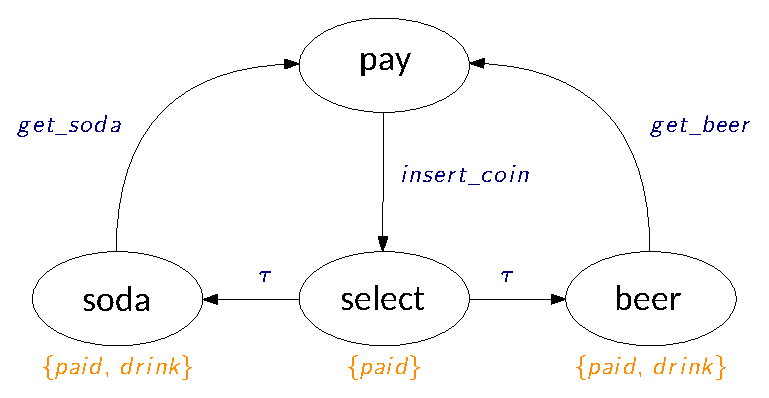
\includegraphics[width=\linewidth]{resources/TS.eps}
    \captionof{figure}{Distributeur de boissons \protect \cite{PMC}}% \protect \cite{DBLP:books/daglib/0020348}}
    \scriptsize
    \begin{columns}
      \begin{column}{0.65\textwidth}
        \begin{itemize}
          \item $ S = \{ pay, \, select, \, beer, \, soda \}$
          \item $ A = \{ insert\_coin,\, \tau,\, get\_soda,\, get\_beer\}$
        \end{itemize}
      \end{column}
      \begin{column}{0.35\textwidth}
        \begin{itemize}
          \item $AP = \{ paid, \, drink \}$
        \end{itemize}
      \end{column}
    \end{columns}
\end{frame}

\begin{frame}{Chemins}
Un chemin d'un système de transition est une succession d'état possible résultant de l'exécution de ce système.
\begin{itemize}
  \item \textbf{\color{fibeamer@orange}Idée}: pas d'états terminaux $\implies$
    chemins infinis.
\end{itemize}
\begin{definition}[Chemin d'un TS]
  Soit $\mathcal{T} = (S, A, \rightarrow, AP, L)$, un TS.
  $\pi = s_0 s_1 s_2 s_3 \dots$ est un \textit{chemin de $\mathcal{T}$} ssi
  pour tout $i \in \mathbb{N}$, il existe une action $\alpha \in A$ telle que
  $s_i \xrightarrow{\alpha} s_{i+1}$, avec $s_i, s_{i+1} \in S$. \\
  L'ensemble des chemins (infinis) $\pi = s_0s_1\dots$ commençant en l'état $s$ (i.e., tels que $s_0 = s$) est dénoté par $Paths(s)$.

\end{definition}

\end{frame}

\begin{frame}{Traces}
    Les traces d'un système de transition sont des mots infinis sur l'alphabet $2^{AP}$ formés lors de l'exécution du système. \\
\begin{definition}[Traces]
  Soit $\mathcal{T} = (S, A, \rightarrow, AP, L)$, un TS. La trace du chemin $\pi = s_0s_1 \dots$ est donné par \[trace(\pi) = L(s_0)L(s_1)\dots\]
  Dès lors, soit $s \in S$, un état de $\mathcal{T}$, les traces du système
  provenant de l'état $s$ est donné par \[Traces(s) = \{ trace(\pi) \; | \; \pi \in
  Paths(s) \}\]
\end{definition}
\end{frame}

\begin{frame}{Chemins et Traces}{Exemple}
    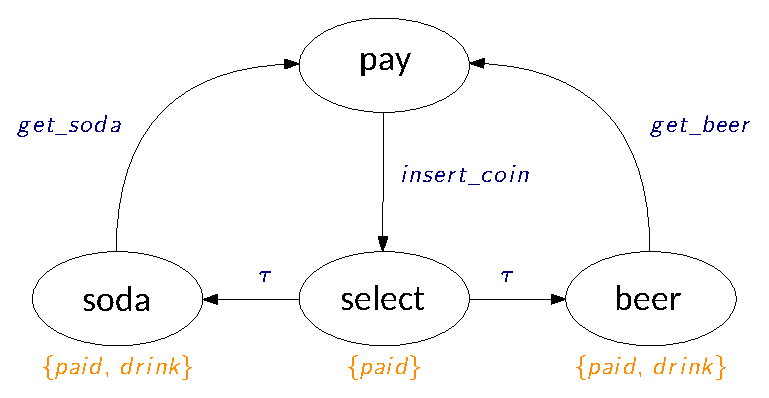
\includegraphics[width=\linewidth]{resources/TS.eps}
    \captionof{figure}{Distributeur de boissons \protect \cite{PMC}}% \protect \cite{DBLP:books/daglib/0020348}}
    \scriptsize
    \begin{itemize}
      \item $\pi = pay\; select \; soda \; pay \; select \; beer \; \dots \in Paths(pay)$
      \item $\{paid\}\{drink\}\{paid\}\{drink\} \dots = trace(\pi) \in Traces(paid)$
    \end{itemize}
\end{frame}

\begin{frame}[allowframebreaks]
        \frametitle{References}
      \printbibliography
\end{frame}

\end{document}
